\documentclass[10pt]{article}

%\bibliographystyle{plain}
\bibliographystyle{abnt-alf}

%Fontes
%\usepackage{pslatex}
%\usepackage{palatino}

\usepackage[brazil]{babel}
\usepackage[latin1]{inputenc}
\usepackage[T1]{fontenc}
\usepackage{graphicx}
\usepackage{amsmath,amssymb,amsbsy,amsthm,ae,aecompl}
\usepackage{url}

%Espa�amento 1.5
\usepackage{setspace}
%\onehalfspacing
\doublespacing


\title{Cria��o de uma biblioteca para HasCASL\\
Proposta de Mestrado}
\author{Glauber M�dolo Cabral -- Orientando\\
Prof. Dr. Arnaldo Vieira Moura -- Orientador}
\date{Setembro de 2007}

\begin{document}

\maketitle

%Resumo
\begin{abstract}
CASL � uma linguagem de especifica��o alg�brica criada para ser um padr�o. Atrav�s de exten��es e restri��es a CASL, cria-se uma fam�lia de linguagens que formam um arcabou�o de especifica��o alg�brica. A exten��o que possui elementos de l�gica de segunda ordem , chamada HasCASL, permite a especifica��o de programas funcionais com elementos muito parecidos com os presentes na linguagem de programa��o Haskell. Embora CASL j� possua uma biblioteca de especifica��es prontas, HasCASL ainda carece de tal biblioteca. Dado que uma linguagem s� � vastamente utilizada quando permite o reuso de c�dido, a presente proposta visa � cria��o de uma biblioteca para HasCASL baseada na biblioteca Prelude, da linguagem funcional Haskell. Prelude ser� tomada como base a fim de facilitar a gera��o de c�digo execut�vel a partir de uma especifica��o em HasCASL, j� que os elementos utilizados encontrar�o correspondentes na biblioteca Prelude.
\end{abstract}

%Corpo
\section{Introdu��o}
CASL � uma linguagem de especifica��o alg�brica criada com o intuito de se tornar padr�o. Esta linguagem permite exten��es e restri��es que originam uma fam�lia de linguagens de especifica��o, formando um arcabou�o para especifica��o alg�brica. A linguagem HetCASL (\textit{Heterogeneous CASL}) permite a integra��o dos m�dulos escritos na demais linguagens, tornando o arcabou�o capaz de suportar diversos paradigmas de programa��o, tais como: especifica��o de aspectos funcionais e reativos de sistemas; programa��o funcional e imperativa; l�gicas de primeira e segunda ordem, modal, temporal e computacional.

Os programas escritos na fam�lia de linguagens de CASL, unidos usando-se HetCASL, podem ser formalmente provados atrav�s da ferramenta Hets. Esta ferramenta, escrita na linguagem funcional Haskell, possui conex�o com os provadores de teorema SPASS e Isabelle, e trasforma as demais linguagens em c�digos que podem ser provados atrav�s destes dois provadores.

Uma linguagem de especifica��o, assim como acontece nas linguagens de programa��o, precisa de bibliotecas com especifica��es comuns j� provadas. Dessa forma, o reuso do c�digo permite que o foco do problema seja atacado sem perda de tempo com partes comuns j� realizadas em outros projetos. Embora CASL j� apresente tal biblioteca, HasCASL ainda n�o possui uma biblioteca com elementos de l�gica de segunda ordem.

A presente proposta tem o intuito de criar tal biblioteca, de forma a colaborar com o aumento no uso da linguagem HasCASL. Pretende-se partir da biblioteca Prelude, de Haskell, de forma que a biblioteca criada contenha todos os tipos definidos na Prelude, ajudando no mapeamento de especifica��es para c�digos execut�veis em Haskell.

Neste documento, a Se��o 2 descreve a linguagem de especifica��o alg�brica CASL, que � extendida e d� origem � linguagem de especifica��o alg�brica HasCASL, descrita na Se��o 3. A Se��o 4 descreve a linguagem de programa��o funcional Haskell, cuja biblioteca Prelude ser� uma das bases do projeto. A Se��o 5 descreve a linguagem HetCASL e a ferramenta Hets; esta �ltima ser� utilizada pra provar formalmente a biblioteca, atrav�s do provador Isabelle, descrito na Se��o 6. A Se��o 7 descreve os objetivos desta proposta e o cronograma de atividades � apresentado na Se��o 8.

%Arrumar: PODEM-SE
\section{CASL}
A linguagem de especifica��o alg�brica CASL surgiu como produto de uma iniciativa internacional para obter uma linguagem �nica de especifica��o que pudesse abranger o maior n�mero de constru��es conhecidas. Esta se��o descreve a linguagem CASL e est� baseada em \cite{Astesiano2002}.

 Com poucas exce��es, as caracter�sticas de CASL est�o presentes de alguma forma em outras linguagens de especifica��o alg�brica. Por�m, uma �nica linguagem n�o serve a todos os prop�sitos desejados: algumas caracter�sticas sofisticadas requerem paradigmas de programa��o espec�ficos e aplica��es especiais; j� m�todos de prototipa��o e gera��o de especifica��es funcionam apenas na aus�ncia de certas caracter�sticas. Por exemplo, reescrita de termos requer especifica��es com axiomas equacionais (com quantificadores ou n�o).

Desta, forma, CASL foi constru�da de forma a ser o n�cleo de uma fam�lia de linguagens: algumas sub-linguagens s�o obtidas atrav�s de restri��es sem�nticas ou sint�ticas, enquanto extens�es s�o criadas para dar suporte a v�rios paradigmas de programa��o. A cria��o da linguagem levou em conta extens�es previamente planejadas, tal qual a que suporta fun��es de segunda ordem. Assim, CASL est� dividida em v�rias partes que podem ser entendidas e usadas separadamente, a saber:
\begin{itemize}
\item Especifica��es B�sicas: cont�m declara��es (de tipos e opera��es), defini��es (de opera��es) e axiomas (relacionando as opera��es);
\item Especifica��es Estruturais: permitem que as Especifica��es B�sicas sejam combinadas para formar especifica��es maiores ; 
\item Especifica��es Arquiteturais: definem como devem ser separadas as v�rias especifica��es na implementa��o, de forma que o reuso de especifica��es dependentes entre si seja poss�vel;
\item Especifica��es de Bibliotecas: definem conjuntos de especifica��es, com constru��es que permitem controle de vers�o e de bibliotecas distribu�das pela Internet.
\end{itemize}

As Especifica��es Estruturais s�o independentes das Especifica��es B�sicas; dessa forma, pode-se criar sub-linguagens ou extens�es de CASL apenas restringindo ou extendendo as constru��es das Especifica��es B�sicas, sem que seja necess�rio alterar os demais tipos. A seguir, descreve-se, sucintamente, as cosntru��es mais importantes das Especifica��es B�sicas.

\subsection{Especifica��es B�sicas}
Uma Especifica��o B�sica denota uma classe de modelos que s�o estruturas poli-sortidas parciais de primeira ordem; ou seja, �lgebras poli-sortidas com fun��es parciais e totais e com predicados. Estes modelos s�o classificados por assinaturas, as quais listam: nomes de tipos, de fun��es (parciais e totais) e de predicados; e, tamb�m, defini��es (ou perfis) de fun��es e predicados.

As especifica��es possuem: declara��es, que introduzem componentes da assinatura (opera��es, ou fun��es, e predicados); e axiomas, que definem propriedades sobre as estruturas que devem servir de modelos para a especifica��o. As opera��es podem ser declaradas totais (usando-se `->') ou parciais(usando-se `->?'), e pode-se atribuir �s mesmas propriedades comuns, tais como a associatividade, evitando a necessidade de axiomatizar tais propriedades.

Opera��es parciais s�o uma maneira simples de tratar erros (como divis�o por zero) e a propaga��o dos mesmos � direta, de tal forma que sempre que um argumento de uma opera��o n�o � definido, o resultado da opera��o tamb�m n�o � definido. Os erros e exce��es tamb�m podem ser tratados por super-tipos de erros e sub-tipos. O dom�nio de uma fun��o parcial pode ser definido como um sub-tipo do tipo do argumento da fun��o, de forma a tornar esta fun��o parcial uma fun��o total sobre o sub-tipo. As fun��es podem ser declaradas totais em sua defini��o, ao inv�s de tratar a totalidade nos axiomas.

Os predicados s�o parecidos com opera��es, mas n�o possuem tipo de retorno; apenas o tipo dos par�metros � declarado. Eles podem ser declarados e definidos ao mesmo tempo, ao inv�s de terem suas declara��es e defini��es em se��es separadas.

Os axiomas s�o escritos em l�gica de primeira ordem sobre f�rmulas at�micas. As vari�veis a serem usadas nos axiomas podem ser declaradas globalmente, antes dos axiomas; ou podem ser declaradas localmente em rela��o a uma lista de f�rmulas;ou, ainda, podem ser declaradas para cada f�rmula, usando quantifica��o expl�cita.

CASL permite que sejam inclu�das anota��es nos axiomas, colocando-se a anota��o entre `\%(' e `)\%', de forma que eles possam ser facilmente referenciados ou utilizados por ferramentas; os coment�rios s�o inclu�dos ap�s `\%\%'.

As assertivas de defini��o s�o utilizadas para indicar, explicitamente, quando determinado termo est� definido ou n�o. A defini��o de um termo via assertiva � equivalente a uma igualdade existencial do termo a ele mesmo. Uma igualdade existencial, declarada usando-se `=e=', entre dois termos do mesmo tipo � v�lida quando os dois termos est�o definidos e s�o iguais; uma igualdade forte, declarada usando-se `=', � v�lida, tamb�m, quando os dois termos est�o indefinidos. A interpreta��o das f�rmulas segue a l�gica de primeira ordem com dois valores (verdadeiro e falso). Existe, ainda, a assertiva de pertin�ncia de sub-tipo, indicada por `in', que cria um predicado relacionando a pertin�ncia de um elemento a um tipo. Como regra, � aconselh�vel usar equa��es existenciais quando definindo condi��es e propriedades e usar equa��es fortes quando definindo fun��es parciais de forma indutiva.

Em CASL, usa-se sem�ntica LOOSE para Especifica��es B�sicas, ou seja, todas as estruturas que satisfazem os axiomas s�o selecionadas como modelos; esta sem�ntica � interessante durante a an�lise de requisitos, de forma que estes �ltimos sejam abrangentes.

Pode-se declarar um tipo de dado como livre, alterando a sem�ntica LOOSE para a sem�ntica inicial. Desta forma, valores de um mesmo tipo que diferem apenas na sequ�ncia da aplica��o dos seus construtores s�o tratados como elementos diferentes deste tipo.

A terceira sem�ntica permitida em CASL for�a os tipos de dados a serem gerados apenas pelos seus construtores. Isto elimina a confus�o entre termos, ou seja, a menos que axiomas forcem uma igualdade, os termos s�o todos diferentes entre si. Esta reintrodu��o de confus�o entre termos � poss�vel atrav�s de axiomas.

As declara��es de tipos s�o as �nicas em que a visibilidade n�o � linear. Em todo o restante das especifica��es, um tempo s� pode ser utilizado depois de ser declarado.

\section{HasCASL}
Esta se��o apresenta a linguagem HasCASL baseando-se em \cite{Schroder}. A defini��o formal da linguagem encontra-se em \cite{Schr�derEtAl03}.

A linguagem HasCASL � uma extens�o de CASL, anteriormente descrita, com conceitos de l�gica de segunda ordem tais como tipos que s�o fun��es, polimorfismo e construtores de tipos. HasCASL foi criada de forma que a linguagem de programa��o funcional Haskell seja seu sub-conjunto; dessa forma, torna-se poss�vel transformar uma especifica��o em HasCASL em um programa Haskell de uma forma mais simples. Como citado anteriormente, para extender CASL � necessario, apenas, extender ou alterar a Especifica��o B�sica, sem que seja necess�rio alterar os outros tr�s tipos de especifica��o.

A l�gica de segunda ordem tradicional n�o permite os tipos e fun��es recursivas amplamente usados em linguagem funcional. HasCASL tenta resolver o problema sem utilizar sem�ntica denotacional, fazendo emergir uma l�gica interna �s $\lambda$-abstra��es sem que esta l�gica seja um conceito primitivo da linguagem. Dessa forma, mant�m-se a linguagem pr�xima a CASL e, ao mesmo tempo, com as propriedades desejadas de l�gica de segunda ordem.

As senten�as em HasCASL diferem de CASL em dois aspectos:
\begin{itemize}
\item Os quantificadores (universal, existencial e unicamente existencial) podem ser aplicados sobre as vari�veis de tipo e possuem restri��es de sub-tipos;
\item Os predicados de CASL s�o substitu�dos por termos do tipo \textit{unit}.
\end{itemize}

Diferentemente das linguagens de programa��o funcional, os opera��es polim�rficos precisam ser explicitamente instanciados, uma vez que ainda n�o est� claro, teoricamente, como se relacionam a resolu��o de sobrecarga de sub-tipos e a instancia��o impl�cita.

Como HasCASL tenta manter-se o mais pr�ximo de CASL, sua sem�ntica tamb�m � baseada em teoria dos conjuntos. Para que as assinaturas de segunda ordem sejam modeladas nesta sem�ntica, � usada a no��o de modelo Henkin intensional. Neste modelo, os tipos de fun��es s�o interpretados por conjuntos arbitr�rios equipados com uma opera��o de aplica��o do tipo apropriado (em oposi��o a um tipo parcial $s->?t$ ser interpretado pelo conjunto completo de todas as fun��es parciais de $s$ em $t$). A interpreta��o dos $\lambda$-termos � parte da estrutura do modelo ao inv�s de ser apenas um axioma existencial.

O modelo intensional tem algumas vantagens, entre as quais: eliminar os problemas de completude; permitir modelos iniciais de assinaturas que contenham fun��es parciais; e permitir que a sem�ntica operacional das linguagens de programa��o funcional seja aplicada, ao inv�s de usar diretamente a l�gica de segunda ordem.
Ao contr�rio de Haskell, na qual a avalia��o de fun��es � pregui�osa, a avalia��o de fun��es em HasCASL � estrita, ou seja, argumentos indefinidos sempre resultam em valores indefinidos. Uma maneira de emular a avalia��o pregui�osa, na qual � permitido que fun��es deixem de avaliar argumentos n�o utilizados internamente a fim de retornar valores definidos mesmo na presen�a de argumentos indefinidos, � mover os par�metros para tipos unit�rios ($unit ->? a$).

Os tipos s�o definidos pelo uso da palavra reservada $type$, que pode ser precedida pelos qualificadores $free$ e $generated$, como em CASL. Defini��es de tipo que possuam tipos de fun��es como argumentos de construtores e recurs�o apenas no lado direito da seta devem ser realizadas com a palavra-reservada $cofree$; com recurs�o em ambos os lados da seta, os tipos devem ser definidos com $free$.

Fun��es recursivas, por sua vez, s�o definidas utilizando a abreviatura $op \; f:t = rec \, \alpha$ que equivale a declarar a opera��o $op \; f:t$ e adicionar o axioma $f=Y(\lambda f:t.a)$, onde Y � o operador de ponto fixo.

\section{Haskell}
Esta se��o apresenta algums elementos sint�ticos da linguagem Haskell. As informa��es aqui fornecidas, bem como conceitos mais aprofundados, podem ser obtidos em materiais encontrados na internet \cite{learnHaskell} ou em livros \cite{Thompson1999}.

Haskell � uma linguagem de programa��o funcional pura, fortemente tipificada e com avalia��o pregui�osa (\textit{lazy evaluation}) que surgiu da necessidade de padroniza��o no campo das linguagens funcionais. A linguagem � funcional porque implementa os conceitos do $\lambda$-C�lculo; logo, a programa��o � feita atrav�s de aplica��es de fun��es ou computa��es. A linguagem � fortemente tipificada, ou seja, os tipos de fun��es e valores precisam ser definidos explicitamente ou o compilador ir� tentar resolver o tipo para o mais abrangente poss�vel no contexto atual.
%Comentar sobre o desaparecimento do conceito de sequenciamento de opera��es

Os conceitos de avalia��o pregui�osa e avalia��o estrita (\textit{strict evaluation}) est�o relacionados com a interpreta��o dos par�metros de uma fun��o. Uma linguagem com avalia��o estrita avalia todos os par�metros da chamada de uma fun��o antes de executar o corpo da fun��o chamada. No caso de Haskell, os par�metros de uma fun��o s�o avaliados apenas quando tornam-se necess�rios para a execu��o da fun��o.

A linguagem � pura porque n�o permite que a aplica��o de uma fun��o altere o estado do sistema (a menos das partes envolvidas nos c�lculos do qual a aplica��o depende). Algumas linguagens funcionais s�o ditas n�o-puras porque permitem que, al�m de efetuar a aplica��o de fun��es, um programa defina a��es tipicamente de linguagens imperativas, como exibir algo em tela ou salvar um conte�do em um arquivo. Estas a��es causam efeitos colaterais, alterando o mundo real.

O mundo real pode ser entendido como tudo que est� diretamente ligado ao sistema em que o programa est� rodando; os efeitos colaterais, por sua vez, s�o todos os efeitos que n�o sejam o c�lculo de fun��es. Haskell permite executar a��es que alterem o mundo real atrav�s de uma entidade matem�tica chamada \textit{m�nada}. As m�nadas seq�enciam computa��es passando, implicitamente, o estado atual do mundo real; isto permite que os efeitos colaterais n�o interfiram no c�digo do programa.

Pode-se definir uma fun��o, em Haskell, diretamente como se faria em $\lambda$-C�lculo, com tipos ou n�o. Uma vantagem de se utilizar uma linguagem de programa��o � poder reutilizar m�todos definidos atrav�s de nomes dados aos mesmos. Nomeia-se, ent�o, uma fun��o cujo corpo est� escrito em $\lambda$-C�lculo a fim de reutiliz�-la. Como o tipo dos elementos n�o foi declarado, o compilador ir� calcular os tipos de acordo com o contexto. Para definir-se o tipo de uma fun��o, deve-se escrever o nome da mesma seguido por ``::'' e pela seq��ncia de tipos de cada par�metro, separados por ``->'', com associa��o � direita.

Dessa forma, sem se afastar muito do $\lambda$-C�lculo, � poss�vel escrever programas em Haskell. Contudo, na maioria dos casos, as fun��es s�o definidas de acordo com a sintaxe de Haskell, por ser mais pr�tica e f�cil. Uma fun��o � definida por um nome seguido por uma seq��ncia de par�metros separados do corpo da fun��o pelo sinal de ``=''.

Faz-se necess�rio diferenciar uma fun��o de um operador. Uma fun��o, em Haskell, � sempre definida de forma prefixa; um operador tem sua defini��o infixa. Uma fun��o prefixa pode ser usada de forma infixa colocando-a entre crases; um operador, por sua fez, pode ser utilizado de forma prefixa colocando-o entre par�nteses.

Outra caracter�stica explorada � a coincid�ncia de padr�es (\textit{pattern matching}). Uma fun��o para calcular o fatorial de um inteiro pode ser definida, utilizando-se coincid�ncia de padr�es, como se segue:
\begin{verbatim}
fat :: Int-> Int
fat 1 = 1
fat x = x * fat(x-1)
\end{verbatim}

Cada chamada � fun��o \textit{fat} percorrer�, em ordem, as duas defini��es da fun��o. Se o par�metro for o inteiro 1, ele ser� retornado; caso contr�rio, ser� feita uma chamada recursiva � fun��o com o par�metro decrescido de uma unidade.

Haskell permite a cria��o de bibliotecas, que s�o chamadas de m�dulos e s�o criadas com a palavra-chave \textit{module}. A linguagem possui uma biblioteca padr�o chamada \textit{Prelude}, na qual s�o definidas fun��es b�sicas que operam sobre os tipos primitivos: \textit{Int}, \textit{Bool}, \textit{Char}, \textit{Float}; e sobre uplas (seq��ncias de valores entre par�nteses) e listas definidas sobre os tipos primitivos.

Haskell, como as demais linguagens funcionais, trabalha com listas como ferramenta principal para representa��o de dados. Pode-se criar listas de tipos primitivos, listas de uplas, listas de listas, listas de fun��es; todos os elementos da lista, contudo, precisam ser de tipos id�nticos. A ordem e a quantidade de elementos dentro de uma lista tamb�m s�o importantes para efeito de igualdade. A lista $[1,2]$ n�o � igual � lista $[2,1]$ e ambas s�o diferentes das lista $[1,1,2]$.

Dois operadores b�sicos para se manipular listas s�o o operador ``:'' (constru��o) e o operador ``++'' (concatena��o). Uma lista sempre � constru�da a partir de uma lista vazia unindo-se a esta o elemento desejado atrav�s do construtor de listas; dessa forma, as seguintes listas s�o eq�ivalentes: $[1,2,3] = 1:2:3:[] = 1:2:[3] =  1:[2,3 $. Para que se possa concatenar duas listas, elas precisam ser do mesmo tipo. As listas $[1,2,3]::[Int]$ e $[4,5,6]::[Int]$ podem ser concatenadas por $[1,2,3]++[4,5,6]$, produzindo a lista $[1,2,3,4,5,6]$.

Uma ferramenta fundamental da linguagem Haskell � a defini��o de Tipos de Dados. Define-se um tipo com a palavra-chave \textit{data} seguida do nome do tipo e do sinal de igual; em seguida, listam-se os elementos que comp�em o tipo (os construtores), separados por ``|''. Tanto o nome do tipo quanto dos construtores devem iniciar-se com letra mai�scula. Um construtor pode ser apenas um nome ou um nome seguido de tipos ou vari�veis de tipos; as vari�veis servem para definir tipos polimorfos e devem ser unidas, atrav�s de par�nteses, ao nome do construtor, de forma a evitar ambig�idade.

Por fim, pode-se incluir a especifica��o de um tipo de dado em uma biblioteca. A declara��o  deve exportar, em sua defini��o, todos os m�todos definidos pela especifica��o, garantindo a integridade do tipo de dado e as propriedades provadas para o tipo em quest�o. Os nomes devem ser exportados no formato \textit{m�dulo.opera��o}, de forma que n�o gere conflitos de nomes com vari�veis de outros pacotes presentes no escopo atual. Isto � uma limita��o da linguagem que j� est� sendo aprimorada pelo grupo de trabalho do compilador \textit{GHC} \cite{ghc}.

\section{Especifica��es Heterog�neas: HetCASL e Hets}
Na �rea de m�todos formais e l�gica s�o utilizadas diversas l�gicas distintas porque, atualmente, n�o se conhece uma maneira de combin�-las de forma a obter uma �nica l�gica que se preste a todos os usos desejados. Especificar sistemas grandes, ent�o, exige o uso de especifica��es heterog�neas porque determinados aspectos s�o melhor abordados por uma l�gica espec�fica. Uma especifica��o heterog�nea possui uma interoperabilidade formal entre as linguagens, de forma que cada linguagem possua seu m�todo de prova e que todas as provas sejam consistentes quando vistas do ponto de vista da especifica��o heterog�nea.

As diversas sub-linguagens e extens�es de CASL s�o �nidas pela linguagem ``Heterogeneous CASL (HetCASL)''\cite{MossakowskiWeb}, que possui as constru��es estruturais de CASL. HetCASL estende a propriedade da sem�ntica de CASL ser independente de institui��o com constru��es que indicam a rela��o entre a tradu��o entre especifica��es que ocorre em conjunto com a tradu��o entre l�gicas. Vale ressaltar que ``HetCASL'' preserva o fato de as l�gicas individualmente usadas pelas especifica��es s�o ortogonais a CASL.

A ferramenta ``Heterogeneous Tool Set (Hets)''\cite{MossakowskiWeb} � um analisador sint�tico e um gerenciador de provas para HetCASL, implementado em Haskell, que combina as v�rias ferramentas de provas existentes para cada uma das l�gicas individuais utilizadas nas diversas sub-linguagens e extens�es de CASL. Hets baseia-se em um grafo de l�gicas e linguagens, provendo uma sem�ntica clara para especifica��es heterog�neas bem como um c�lculo de provas. 

Cada l�gica do grafo � representada por um conjunto de tipos e fun��es em Haskell. A sintaxe e a sem�nticas das especifica��es heterog�neas em HetCASL e as suas respectivas implementa��es s�o parametrizadas por um grafo de l�gicas arbitr�rio dentro da ferramenta Hets. Isto permite que a implementa��o da ferramenta e dos m�dulos para cada l�gica sejam facilmente gerenci�veis do ponto de vista de engenharia de software.

Entre as diversas l�gicas suportadas por Hets, s�o de interesse: HasCASL, Haskell, SPASS e Isabelle. As d�as �ltimas s�o as �nicas que possuem provadores, a saber: SPASS \cite{WBH+02} � um provador autom�tico de teoremas para l�gicas de primeira ordem com igualdade; Isabelle \cite{Nipkow-Paulson-Wenzel:2002} � um provador semi-autom�tico de teoremas para l�gicas de segunda ordem. As demais l�gicas s�o provadas atrav�s de tradu��es entre elas mesmas e uma das duas l�gicas com provadores.

A estrutura de provas em Hets baseia-se no formalismo de grafos de desenvolvimento \cite{Mossakowski2006}, amplamente utilizado para especifica��es de sistemas industriais. A estrutura de grafos permite a visualiza��o direta da estrutura da especifica��o e facilita o gerenciamento de especifica��es com muitas sub-especifica��es.

Um grafo de desenvolvimento consite em um conjunto de n�s (correspondentes a especifica��es completas ou trechos de especifica��es) e um conjunto de arcos chamados arcos de defini��o que indicam a dependencia entre as v�rias espeficica��es e suas sub-especifica��es. A cada n� est�o associados uma assinatura e um conjunto de axiomas locais, sendo que estes �ltimos s�o herdados pelos n�s dependentes atrav�s dos arcos de defini��o. Diferentes tipos de arcos s�o utilizados para indicar quando h�, ou n�o, mudan�a da l�gica entre dois n�s.

Um segundo tipo de arco, os arcos de teorema, s�o utilizados para postular rela��es entre diferentes teorias, servindo para representar as necessidades de prova que surgem durante o desenvolvimento. Os arcos de teorema podem ser globais ou locais (representados por arcos de formas distintas no grafo): os arcos globais indicam que todos os axiomas do n� fonte s�o v�lidos no n� alvo; os arcos locais indicam que apenas os axiomas do n� fonte s�o v�lidos no n� alvo.

Os arcos de teoria globais s�o decompostos em arcos mais simples (globais ou locais) atr�v�s do c�lculo de prova para gafos de desenvolvimento. Os arcos locais podem ser provados tranformando-os em alvos locais de prova, os quais podem ser provados utilizando o c�lculo de prova da l�gica representada no n�.

Abaixo est�o reproduzidos dois trechos de c�digos utilizados pela ferramentas Hets. O primeiro, escrito na l�gica CASL, extende um tipo previamente definido (AllenHayes), incluindo defini��es e senten�as; estas �ltimas decorrem das primeiras e geram obrigatoriedade de prova para as senten�as:
\begin{verbatim}
logic CASL
spec ConstructPointsFO[AllenHayes] = %def
  preds __ __ Equi __ __, __ __ Less __ __: Elem x Elem x Elem x Elem 
  forall x,y,z,u:Elem
  . x y Equi z u <=> z M y /\ z M u /\ z M u
  . x y Less z u <=> x M y /\ z M u /\ (exists v:Elem . x M v /\ v M u)
then %implies
  forall x,y,z,u:Elem
  . x M y => x y Equi x y
  . x y Equi z u => z u Equi x y
\end{verbatim}


O segundo exemplo, escrito na l�gica HasCASL, especifica uma interface, declarando um predicado vis�vel nesta interface e definindo seu funcionamento atrav�s de uma senten�a:
\begin{verbatim}
logic HasCASL
view FlowOfTime_In_ConstructPointsFromIntervals[AllenHayes]:
  FlowOfTime to
  { ConstructPointsFromIntervals[AllenHayes] then %def
    pred __ < __ : Inst X Inst
    forall X,Y:Inst . X < Y <=> exists x,y,u,v:Elem
      . x M y /\ u M v /\ X = eqcl(x,y)/\ Y = eqcl(u,v) 
        /\ x y Less u v}
= sort Elem |-> Inst
\end{verbatim}

O c�digo do qual os trechos foram retirados origina o grafo de desenvolvimento da Figura~\ref{grafo}.

\begin{figure}[ht] 
 \centering 
 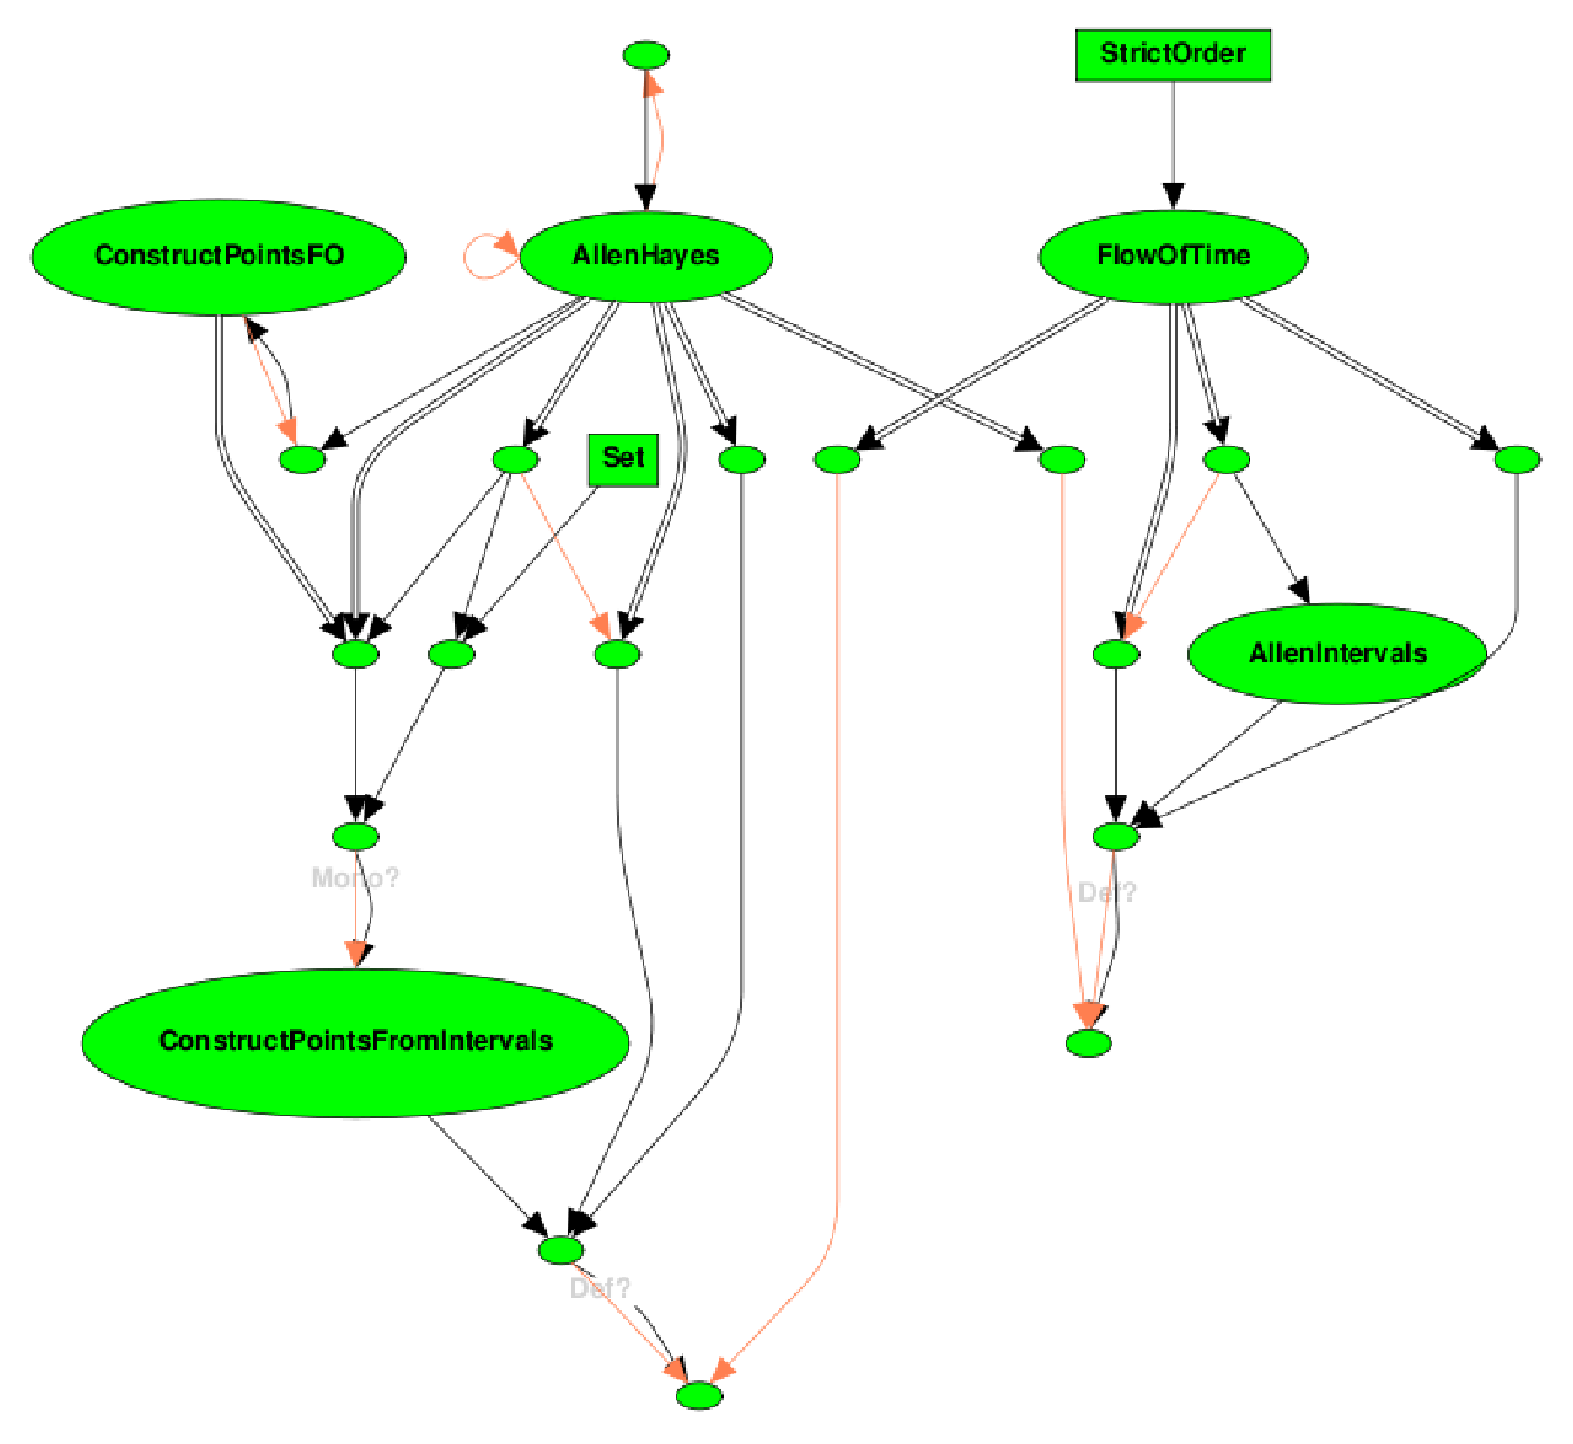
\includegraphics[width=0.9\textwidth]{grafo} 
 \caption{Exemplo de grafo de desenvolvimento} 
 \label{grafo} 
\end{figure}
\section{Isabelle}
Esta se��o descreve o provador de teoremas Isabelle baseando-se na documenta��o presente em seu \textit{site} na Internet \cite{IsabelleSite}; uma descri��o completa pode ser encontrada no manual do provador \cite{Nipkow-Paulson-Wenzel:2002}.

Isabelle � um provador de teoremas gen�rico que permite o uso de v�rias l�gicas como c�lculo formal na prova de teoremas. Hets utiliza Isabelle para provar teoremas em l�gica de segunda ordem, mas o provador permite , por exemplo, o uso de teoria de conjuntos axiomatizada, dentre outras l�gicas. O suporte a v�rias l�gicas � uma das caracter�sticas de destaque da ferramenta.

O provador possui um excelente suporte � nota��o matem�tica: novas nota��es podem ser inclu�das utilizando-se s�mbolos matem�ticos comuns e as provas podem ser descritas de forma estruturada ou, mais facilmente, como seq��ncia de comandos. As defini��es e provas podem incluir c�digos na linguagem de formata��o TeX, de forma que documentos formatados possam ser gerados diretamente do c�digo fonte.

A maior limita��o de provadores de teorema � a necessidade de grande esfor�o e experi�ncia por parte dos usu�rios para que as provas sejam realizadas. Visando a facilitar este processo, Isabelle possui algumas ferramentas que automatizam alguns trechos de provas, tais como equa��es, aritm�tica b�sica e f�rmulas matem�ticas.

A l�gica de segunda ordem HOL � utilizada na codifica��o das teorias. Sua sintaxe assemelha-se muito �s linguagens de programa��o funcional por ser baseada em c�lculo lambda tipificado. Esta l�gica permite constru��es de tipos de dados, tipos de fun��es e outras constru��es comuns em linguagens funcionais. A traadu��o de HasCASL para HOL � feita pela ferramenta Hets de forma autom�tica.

Isabelle possui uma extens�o, chamada Isar, que permite descrever as provas de forma que tanto humanos possam l�-las como computadores possam interpret�-las facilmente. O provador possui uma extensa biblioteca de teorias matem�ticas j� provadas (por exemplo, nas �reas de �lgebra e Teoria de Conjuntos) e, tamb�m, muitos exemplos de provas realizadas em Verifica��o Formal.

A seguir, apresenta-se a codifica��o em Isar do Teorema de Cantor, que afirma a exist�ncia de mais subconjuntos do que elementos em um conjunto qualquer. O c�digo descreve como a prova deve ser realizada, por�m, poderia ter sido escrito de forma que Isabelle efetuasse uma prova autom�tica.

\begin{verbatim}
theory Cantor imports Main begin

theorem "EX S. S ~: range (f :: 'a => 'a set)"
proof
  let ?S = "{x. x ~: f x}"
  show "?S ~: range f"
  proof
    assume "?S : range f"
    then obtain y where "?S = f y" ..
    then show False
    proof (rule equalityCE)
      assume "y : f y"
      assume "y : ?S" then have "y ~: f y" ..
      with `y : f y` show ?thesis by contradiction
    next
      assume "y ~: ?S"
      assume "y ~: f y" then have "y : ?S" ..
      with `y ~: ?S` show ?thesis by contradiction
    qed
  qed
qed

\end{verbatim}
\section{Proposta}
Um pr�-requisito para o uso pr�tico de uma linguagem de especifica��o � a disponibilidade de um conjunto de especifica��es padr�es previamente dispon�veis \cite{Schroder2006}. A linguagem CASL possui tal conjunto descrito em ``CASL Basic Datatypes'' \cite{Roggenbach:2004:CASL-Libraries}; o documento, ao inv�s de fornecer blocos comuns para reuso como acontece com bibliotecas em linguagens de programa��o, fornece exemplos completos de especifica��es que ilustram o uso de CASL tanto no n�vel das Especifica��es B�sicas quanto das Especifica��es Estruturais.
As especifica��es inclu�das s�o tanto de tipos b�sicos de dados como de especifica��es que expressam propriedades de estruturas. No primeiro caso, est�o presentes tipos de dados simples, como n�meros e caracteres, bem como tipos de dados estruturados, como listas, vetores e matrizes; no segundo caso, est�o inclu�dos estruturas alg�bricas tais como mon�ides e an�is e propriedades matem�ticas como rela��es de equival�ncia e de ordem parcial.

Atualmente, a linguagem HasCASL n�o possui uma biblioteca nos moldes da biblioteca de CASL. Segundo Scr\"oder, os tipos de dados descritos em ``CASL Basic Datatypes'' podem servir como base para a constru��o de uma biblioteca padr�o paras as extens�es de CASL. No caso de HasCASL, sugere-se a inclus�o de novas especifica��es que envolvam caracter�sticas de ordem superior tais como a completude de ordena��es parciais assim como estender os tipos de dados efetuando, antes, a troca da parametriza��o no n�vel das Especifica��es Estruturais pela depend�ncia de tipos. Um exemplo sugerido � a inclus�o de fun��es de ordem superior que operem sobre listas, tais como as fun��es \textit{map}, \textit{filter} e \textit{fold}, utilizando-se especifica��es heterog�neas (usando-se CASL e HasCASL) para maximizar o reuso.

Com base nestas sugest�es, prop�e-se iniciar a cria��o de uma biblioteca para HasCASL tendo como base o documento citado e a biblioteca Prelude, de Haskell. Criar tal biblioteca mostra-se uma tarefa �til, dado que contribuir� para o aumento de uso da linguagem. Como a biblioteca Prelude � uma biblioteca padr�o que deve ser disponibilizada por todo compilador Haskell, transport�-la para HasCASL contribuir� para que as especifica��es sejam mais facilmente mapeadas para c�digo execut�vel em Haskell.

A cria��o de tal biblioteca exige o estudo da teoria de linguagens de programa��o funcional no tocante aos tipos e fun��es de ordem superior e a busca de solu��es para a inclus�o de tais elementos na biblioteca de forma a n�o alterar a bliblioteca de CASL mas, sim, estend�-la.

Os c�digos gerados ser�o verificados atrav�s da ferramenta Hets, gerando provas formais para os mesmos de forma a garantir a corretude de todo o c�digo gerado. Como dito anteriormente, esta ferramenta gerencia as provas e utiliza dois provadores para executar as provas. Faz-se necess�rio, ent�o, aprender a utilizar os dois provadores (SPASS e Isabelle).

Isabelle � o provador que demanda maior trabalho. Sua utiliza��o ser� maior que a do provador SPASS, uma vez que os c�digos que se pretende implementar envolvem os conceitos de ordem superior que s�o provados atrav�s do Isabelle. Como este � um provador semi-autom�tico, ser� necess�ria interven��o manual na prova; isto demanda um aprendizado profundo do sistema, desde a sintaxe utilizada para os arquivos de entrada at� as sa�das geradas pelo provador. O conhecimento dos poss�veis erros gerados torna-se fundamental para que poss�veis erros dos c�digos possam ser procurados e corrigidos.

Uma pos�vel extens�o do trabalho, a ser considerada durante o decorrer da codifica��o, � a especifica��o de alguns outros tipos de dados relacionados a Teoria das Categorias. Isto seria �til na medida em que a base te�rica por tr�s de CASL e de HasCASL est� fortemente ligada a esta teoria. Dessa forma, pode-se iniciar o estudo te�rico deste t�pico com vistas ao in�cio do Doutorado.
\section{Cronograma}
A seguir, apresentam-se as atividades a serem realizadas durante o projeto de mestrado. A Tabela~\ref{tab:cronograma} possui o tempo estimado das atividades:

\begin{enumerate}
\item Cr�ditos obrigat�rios do mestrado; \label{cron:1}
\item Estudo das linguagens HasCASL e CASL, com �nfase nas constru��es de HasCASL e na biblioteca de CASL; \label{cron:2}
\item Estudo da ferramenta Hets e do provador Isabelle; \label{cron:3}
\item Exame de Qualifica��o do Mestrado; \label{cron:4}
\item Estudo da biblioteca Prelude e dos conceitos de l�gica de segunda ordem envolvidos na bilbioteca; \label{cron:5}
\item Implementa��o e prova de corretude da biblioteca para HasCASL. \label{cron:6}
\item Escrita de um artigo para congresso. \label{cron:7}
\item Escrita da disserta��o. \label{cron:8}
\item Defesa e revis�o. \label{cron:9}
\end{enumerate}

{
\small
\begin{table}[hb]
\begin{center}
\begin{tabular}{||c||c|c|c|c|c||c|c|c|c|c|c||c||}

\hline \hline
%% Anos
Atividade
& \multicolumn{5}{c||}{2007} 
& \multicolumn{6}{c||}{2008}
& \multicolumn{1}{c||}{2009} \\ \cline{2-13}

%% Meses
&  3-4 & 5-6 & 7-8 & 9-10 & 11-12 & 1-2 & 3-4 & 5-6 & 7-8 & 9-10 & 11-12 & 1-2 \\ \hline \hline

%% Atividades
\ref{cron:1}  & $\bullet$ & $\bullet$ & $\bullet$ & $\bullet$ & $\bullet$ & & & & & & & \\ \hline 
\ref{cron:2}  & & $\bullet$ & $\bullet$ & & & & & & & & & \\ \hline 
\ref{cron:3}  & & & & $\bullet$ & $\bullet$ & & & & & & & \\ \hline 
\ref{cron:4}  & & & & $\bullet$ & & & & & & & & \\ \hline 
\ref{cron:5}  & & & & & & $\bullet$ & $\bullet$ & & & & & \\ \hline 
\ref{cron:6}  & & & & & & & & $\bullet$ & $\bullet$ & $\bullet$ & & \\ \hline 
\ref{cron:7}  & & & & & & & & & & $\bullet$ & & \\ \hline 
\ref{cron:8}  & & & $\bullet$ & & $\bullet$ & & $\bullet$ & & & & $\bullet$ & \\ \hline 
\ref{cron:9}  & & & & & & & & & & & & $\bullet$ \\ \hline

\end{tabular}
\caption{Cronograma de Atividades: mar�o/2007 at� fevereiro/2009} 
\label{tab:cronograma}
\end{center}
\end{table}
}


\bibliography{Proposta,cofi}

\end{document}

%%% Local Variables: 
%%% mode: latex
%%% TeX-master: t
%%% End: 
